\section{Konstrukcja i sterowanie}
W XXI wieku czołgi stały stały się wielozadaniowymi pojazdami, które można dopasować do niemalże każdego pola bitwy. Cały czas pozostają podstawowymi pojazdami zaczepno-obronnymi wojsk lądowych. Coraz częściej pojazdy tego typu mają budowę modułową, dzięki temu ich naprawa jest dużo prostsza. Stwarza to także możliwość doboru różnorodnego wyposażenia pod kątem konkretnych warunków bojowych \cite{kierunek_rozwoju}. Wprowadza się automatyczne mechanizmy ładowania pocisków aby zmniejszyć czas przeładowania działa i liczebność załogi. Podstawowe segmenty, tzn. wieżyczkę (1), do której zamocowane jest działo(A) oraz kadłub(2), w którym umieszczone są wszystkie podzespoły czołgu, przedstawiono na rysunku \ref{podzal}. 

  \begin{figure}[H]
    \begin{center}
      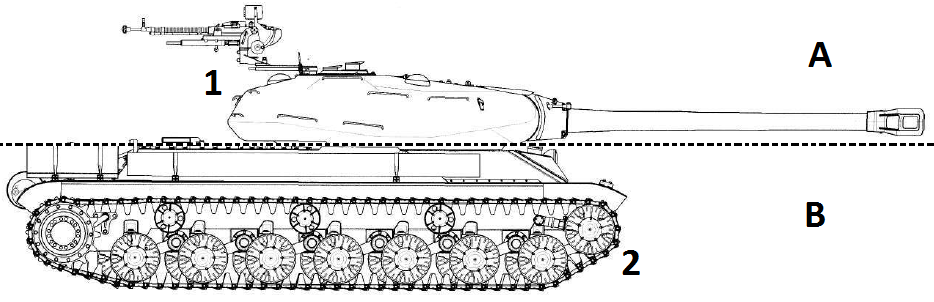
\includegraphics[scale=0.5]{imgs/cz_bud.png}
 	\caption[Czołg \textit{IS-4} - podział]{\small{Radziecki czołg IS-4. Na ilustracji wyróżnione zostały podstawowe segmenty pojazdu : A-wieżyczka, B-kadłub oraz elementy ruchome : 1-działo, 2-gąsiennice.}\footnotemark[12]}
	\label{podzal}
    \end{center}
  \end{figure}
  \footnotetext[12]{\emph{Monografia IS-3}, Publikacja rosyjska, 2010~r.}

\newpage

Wieżyczka (A na ilustracji \ref{podzal}) pojazdu umożliwia kierować ogień w dowolną stronę. Jej budowa pozwala na: obrót wokól osi pionowej o 360 stopni, regulację wychylenia działa (odpowiednio: $x^\circ$ w górę, $y^\circ$ w dół - zgodnie z rysunkiem \ref{wez_czolg}).

  \begin{figure}[H]
    \begin{center}
      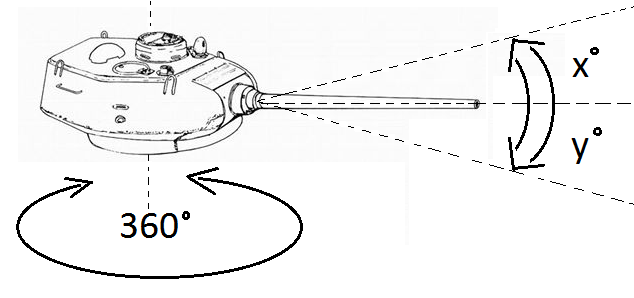
\includegraphics[scale=0.55]{imgs/wiezyczka.png}
 	\caption[Wieżyczka \textit{T-34-85}]{\small{Wieżyczka czołgu T-34-85 wraz z zaznaczonymi możliwymi wychyleniami. Wartości $x$ i $y$ przyjmują różne wartości, w zależności od modelu.}\footnotemark[13]}
	\label{wez_czolg}
    \end{center}
  \end{figure}
  \footnotetext[13]{\emph{Czołg T-34 i inne konstrukcje wozów bojowych II Wojny Światowej}, http://facebook.com/, (data dostępu 28.09.2015r.)} 

Korpus czołgu (B na ilustracji \ref{podzal}) jest jednostką napędową całej konstrukcji. Struktura podwozia najczęściej opiera się na gąsienicach. Ich popularność wynika z tego, że równomiernie rozkładają ciężar na dużą powierzchnię. Dzięki temu pojazd mimo ogromnej masy bardzo dobrze radzi sobie w trudnych warunkach terenowych. Aby zapewnić okrętowi lądowemu zadowalającą zwrotność zdecydowano o rozdzieleniu napędu osobno na prawą oraz lewą gąsienice. Sposób sterowania kierunkiem obrotu poszczególnych stron napędu pokazano na ilustracji \ref{ster}. 

  \begin{figure}[H]
    \begin{center}
      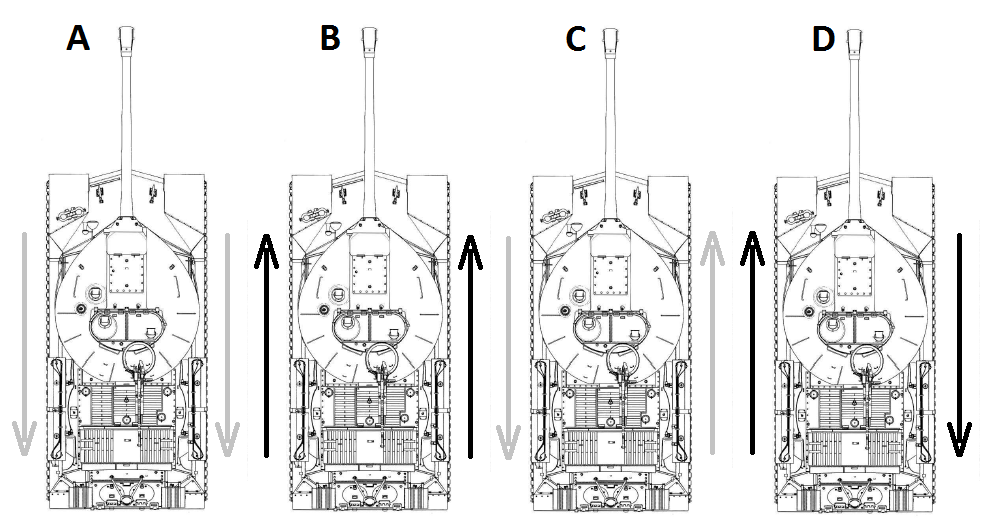
\includegraphics[scale=0.45]{imgs/ster.png}
 	\caption[Czołg \textit{IS-3} - sterowanie]{\small{Ilustracja przedstawia sposób sterowania czołgiem na przykładzie IS-3. Kolejno: A-jazda w tył, B-w~przód, C-w~lewo, D-w~prawo.}\footnotemark[14]}
	\label{ster}
    \end{center}
  \end{figure}
  \footnotetext[14]{\emph{Monografia IS-3}, Publikacja rosyjska, 2010~r.}

\section{Przetwarzanie obrazu}
Obraz cyfrowy, w dalszej części pracy nazywany po prostu obrazem, jest graficzną reprezentacją tablicy, którą można także przedstawić za pomocą funkcji:
\begin{equation}
\label{funkcja_obrazu}
    z = f(x,y), dla: x = 0, 1, 2, ..., N-1; y = 0, 1, 2, ..., M-1
\end{equation}
gdzie:\\
$N$ - szerokość obrazu,\\
$M$ - wysokość obrazu\\
$z$ - wartość funkcji w punkcie.\\
W najprostszym przypadku obrazów czarno-białych wartością wyrażana przez tą funkcję jest stopień szarości każdego piksela (tj. najmniejszej składowej obrazu cyfrowego, charakteryzującej się jednolitą barwą). Obraz składa się wtedy z jednej, dwuwymiarowej tablicy o wymiarach $N$ na $M$.

W przypadku obrazów kolorowych jednak do przedstawienia obrazu stosuje się kilka takich funkcji. Najpopularniejszym sposobem przedstawiania kolorów w grafice komputerowej jest model RGB. Skrót ten tworzą pierwsze litery angielskich nazw kolorów będących bazą w tym modelu: \textit{red} (czerwony), \textit{green} (zielony) oraz \textit{blue} (niebieski), których odpowiednia kombinacja umożliwia uzyskanie każdego koloru. W przypadku wykorzystania tego modelu obraz zapisany jest jako trzy tablice, przechowujące odpowiednio natężenia kolorów czerwonego, zielonego i niebieskiego.

Obrazy, na których będą wykonywane operacje na potrzeby tego projektu będą obrazami rejestrowanymi przez kamerę zamontowaną na robocie, a więc odzwierciedlającymi rzeczywiste otoczenie. Rejestracja rzeczywistego obrazu na postać cyfrową polega na dyskretyzacji obrazu oraz kwantyzacji jasności koloru\cite{Malina}. Dyskretyzacja obrazu rzeczywistego polega na próbkowaniu go w dwóch wymiarach. W każdym polu tabeli, odpowiadającej za jeden kolor, zapisywana jest wartość natężenia danego koloru dla wycinka obrazu rzeczywistego, któremu odpowiada adres danego pola. Rejestrowane natężenie każdego z kolorów jest wartością ciągłą i w celu zapisania jej w pamięci komputera stosuje się kwantyzację, tj. podzieleniu całego zakresu jasności na przedziały i przypisywaniu wartości rejestrowanej do jednego z tych przedziałów. Wynik tej operacji jest najczęściej zapisywany na 8 bitach, a więc posiada wartości od 0 do 255 ($2^8$ daje 256 kombinacji). Pamiętając, że tworzone są trzy tablice, osobna dla każdego z kolorów RGB, a więc dane każdego piksela zapisywane są na $3 x 8 = 24$ bitach. Daje to kombinację $2^{24} = 16777216$ kolorów, czyli ilość przekraczającą już możliwości percepcji ludzkiego oka.

\textit{Celem sztucznego przetwarzania lub analizy obrazu jest takie automatyczne przetworzenie i przeanalizowanie obrazu obiektów lub całego otoczenia systemu zautomatyzowanego, aby uzyskać użyteczną informację na temat interesujących obiektów (...) lub na temat otoczenia, które może wpływać (...) na sterowany automatycznie proces.}\cite{Tadeusiewicz}

Czytając powyższą definicję należy być świadomym, że obraz rzeczywistego otoczenia posiada olbrzymią ilość informacji, w znacznej mierze nadmiarowych, nie mających związku z poszukiwanymi informacjami. Analizowanie obrazów dokonywane w ludzkim mózgu jest dla człowieka czynnością naturalną, ćwiczoną od chwili narodzin. Wydaje się więc być czymś prostym. W rzeczywistości próba powtórzenia tych procesów w sposób sztuczny jest rzeczą niezwykle trudną i złożoną. Cały proces wydobywania informacji obrazu można podzielić na trzy etapy: przetwarzanie, analizę oraz rozpoznawanie.

Przetwarzanie obrazu jest to proces, charakteryzujący się tym, że na jego wyjściu, tak samo jak na wejściu, znajduje się obraz cyfrowy. Operacje te wykonuje się w celu poprawy jakości samego obrazu, uwypukleniu jego cech. Typowymi operacjami należącymi do dziedziny przetwarzania obrazu są np. różnego rodzaju filtracje czy wyostrzanie krawędzi.

Kolejnym procesem jest analiza obrazu będącego wynikiem przetwarzania. Polega ona na zastosowaniu algorytmów, których celem jest wyodrębnienie poszukiwanych danych ilościowych i jakościowych. Na wyjściu otrzymuje się więc nie pełen obraz, z całą nadmiarowością danych, a jedynie informacje użyteczne w danym procesie.

Uzyskane w powyższy sposób informacje wykorzystuje się na ostatnim etapie, tj. w procesie rozpoznawania. \textit{(...) w zadaniu rozpoznawania chodzi o rozpoznawanie przynależności rozmaitego typu obiektów (lub zjawisk) do pewnych klas}\cite{Tadeusiewicz_flasinski}. Algorytm odpowiedzialny za te działania opiera się więc o zbiór cech, których wartości dla danego obrazu są otrzymywane w procesach przetwarzania i analizy obrazu. Następnie wykorzystuje posiadane już reguły (np. zdobyte za pomocą algorytmu uczącego) aby móc w sposób ostateczny scharakteryzować obraz wejściowy.
